\skipnexttoc
\section{Implementation}
\subsection{Architecture}
\begin{frame}
	\frametitlesubs
	\begin{figure}[H]
		\centering
		\bgroup
		\footnotesize\tt
		\tikzset{
			LL/.style={
				draw=black,decorate,
				decoration={snake, segment length=3mm,post}
			},
			>={Latex[width=1mm,length=1mm]},
			every node/.style = {draw, align=center},
		}

		\newcommand{\byty}{-1.3}

		\begin{tikzpicture}
			\node[ellipse,fill=\nodecolor] (source) at (5.3, 3.2) {\textsf{Source}};
			\node[above = of source,star,star points=6,star point ratio=0.8,fill=\nodecolor] (bytecode) {\textsf{bytecode}};
			\coordinate[above = of bytecode] (pt9);
			\coordinate[right = 3.7 of pt9] (pt5);
			\node[rectangle,fill=\nodecolor,below = 0.4 of pt5] (adata) {analyzed data};
			\node[rectangle,text width=3.6cm,align=center,fill=\nodecolor,below = 2 of adata] (cfgduch) {Control Flow Graph\\\& DU~Chain};
			\coordinate[right = 4.3 of adata] (pt6);
			\coordinate[right = 2 of adata] (pt7);
			\coordinate[right = 2 of cfgduch] (pt8);
			\draw[->] (source) -- (bytecode);
			\draw (bytecode) -- (pt9);
			\draw[->] (pt9) -| (adata);
			\draw[->] (adata) -- (cfgduch);
			% \draw[LL,thick,>=latex] (adata) -- (pt7);
			% \draw[LL,thick,>=latex] (cfgduch) -- (pt8);
			\node[fill=yellow!20,rectangle, text width=19\zw,below = -1.6\zw of pt6] (opts){%
				\textcolor{red}{optimizer}\\%
				\begin{itemize}
					\item Constant Folding
					\item Constant Propagation
					\item Dead-code Elimination
					\item Function Inlining
					\item Unreachable Block Removal
					\item Unused Resource Removal
			\end{itemize}};
			\draw[LL,thick,>=latex,->] (adata) -- (opts);
			\draw[LL,thick,>=latex,->] (cfgduch) -- (opts);
			\coordinate[below = 1.3 of opts] (pt2);
			\coordinate[left = 8 of pt2] (pt3);
			\draw[to path = {-| (\tikztotarget)},->] (opts) |- (pt3) |- (adata);
			% \node[draw=none, above] at ($(pt2)!0.5!(pt3)$) {again};
			\node[right = 1.3 of pt2,text width=4.8em,fill=\nodecolor,circle] (optbc) {\textsf{optimized\\bytecode}};
			\draw[->] (pt2) --  (optbc);
		\end{tikzpicture}
		\egroup
		\caption{optimization image}
	\end{figure}
\end{frame}
\subsection{Bytecode}
\begin{frame}
	\frametitlesubs
	\begin{figure}
		\centering
		\begin{tikzpicture}
			\node[text width=13\zw] (sousa) at (0, 0) {Lua VM 5.3のバイトコード\\を操作したい};
			\node[right = .5 of sousa] (arrow) {$\Rightarrow$};
			\node[right = .5 of arrow, text width=13\zw] {バイトコードのdocumentは\\\alert<2->{ない}};
		\end{tikzpicture}
	\end{figure}

	\pause
	\vspace{3\zw}
	\begin{center}
		$\Rightarrow$ \alert{自分で読み解くしかない}
	\end{center}
\end{frame}
\begin{frame}
	\frametitlesubs

	有志の非公式ドキュメント
	\begin{itemize}
		\item Lua VM 5.3 instructions (bytecodeではない)\footnote{\url{https://github.com/dibyendumajumdar/ravi/blob/master/readthedocs/lua_bytecode_reference.rst}}
		\item Lua VM 5.1 reference\footnote{\url{http://luaforge.net/docman/83/98/ANoFrillsIntroToLua51VMInstructions.pdf}}
	\end{itemize}
	\pause

	Lua VM bytecodeを読むためのツール
	\begin{itemize}
		\item \lstinline{luac -l -l luac.out}
		\item \lstinline{xxd -g 1 luac.out | nvim - -R}\pause
		\item ソースコード\footnote{\url{https://www.lua.org/source}}
	\end{itemize}

	\pause
	\begin{center}
		簡単に言うと\alert{\Huge{}気合}
	\end{center}
\end{frame}
\begin{frame}[fragile]
	\frametitlesubs
	\hspace{-.5\zw}
	\begin{minipage}[t]{.34\textwidth}
		\bgroup\footnotesize
		\begin{lstlisting}[numbers=none,language={[5.3]lua}]
print("hello, world!")
		\end{lstlisting}
		\tiny
		\begin{lstlisting}[numbers=none]
 $ luac -l -l luac.out

main <hello.lua:0,0> (4 instructions at 0x16e79e0)
0+ params, 2 slots, 1 upvalue, 0 locals, 2 constants, 0 functions
  1  [1]  GETTABUP     0 0 -1  ; _ENV "print"
  2  [1]  LOADK        1 -2    ; "hello, world!"
  3  [1]  CALL         0 2 1
  4  [1]  RETURN       0 1
constants (2) for 0x16e79e0:
  1  "print"
  2  "hello, world!"
locals (0) for 0x16e79e0:
upvalues (1) for 0x16e79e0:
  0  _ENV    1       0
		\end{lstlisting}
		\egroup
	\end{minipage}
	\begin{minipage}{.01\textwidth}
		\ 
	\end{minipage}
	\begin{minipage}[t]{.64\textwidth}
		\pause
		\bgroup\tiny
		\begin{lstlisting}[numbers=none]
$ xxd -g 1 luac.out
00000000: 1b 4c 75 61 53 00 19 93 0d 0a 1a 0a 04 08 04 08  .LuaS...........
00000010: 08 78 56 00 00 00 00 00 00 00 00 00 00 00 28 77  .xV...........(w
00000020: 40 01 0b 40 68 65 6c 6c 6f 2e 6c 75 61 00 00 00  @..@hello.lua...
00000030: 00 00 00 00 00 00 02 02 04 00 00 00 06 00 40 00  ..............@.
00000040: 41 40 00 00 24 40 00 01 26 00 80 00 02 00 00 00  A@..$@..&.......
00000050: 04 06 70 72 69 6e 74 04 0e 68 65 6c 6c 6f 2c 20  ..print..hello,
00000060: 77 6f 72 6c 64 21 01 00 00 00 01 00 00 00 00 00  world!..........
00000070: 04 00 00 00 01 00 00 00 01 00 00 00 01 00 00 00  ................
00000080: 01 00 00 00 00 00 00 00 01 00 00 00 05 5f 45 4e  ............._EN
00000090: 56                                                                  V
		\end{lstlisting}
		\egroup\normalfont
		\pause
		\begin{center}
			\vspace{1\zw}
			\LARGE
			\alert{???}
		\end{center}
	\end{minipage}
\end{frame}
\begin{frame}[fragile]
	\frametitlesubs
	\begin{center}
		\begin{minipage}[t]{.4\textwidth}
			\bgroup\tiny
			\begin{lstlisting}[numbers=none]
1b 4c 75 61 53 00 19 93 0d 0a 1a 0a 04 08 04 08
08 78 56 00 00 00 00 00 00 00 00 00 00 00 28 77
40 01 0b 40 68 65 6c 6c 6f 2e 6c 75 61 00 00 00
00 00 00 00 00 00 02 02 04 00 00 00 06 00 40 00
41 40 00 00 24 40 00 01 26 00 80 00 02 00 00 00
04 06 70 72 69 6e 74 04 0e 68 65 6c 6c 6f 2c 20
77 6f 72 6c 64 21 01 00 00 00 01 00 00 00 00 00
04 00 00 00 01 00 00 00 01 00 00 00 01 00 00 00
01 00 00 00 00 00 00 00 01 00 00 00 05 5f 45 4e
56
			\end{lstlisting}
			\egroup
		\end{minipage}
	\end{center}
	\pause
	\begin{figure}[h]
		\def\position{(0.1, -1.76)}
		\tikzset{just here/.style = {above right,inner sep=0mm}}
		\centering
		\begin{tikzpicture}[remember picture]
			\useasboundingbox (0.1,-1.76);
			\coordinate (top) at (-3, 2.3);
			\node[above right = .2 of top] (label) {\textcolor{blue}{header block}};
			\coordinate[right = 6.2 of top] (p1);
			\coordinate[below = 0.55 of p1] (p2);
			\coordinate[left = 5.4 of p2] (p3);
			\coordinate[below = 0.28 of p3] (p4);
			\coordinate[left = 0.8 of p4] (p5);
			\draw[blue, dashed, very thick] (top) -- (p1) -- (p2) -- (p3) -- (p4) -- (p5) -- (top);
		\end{tikzpicture}
	\end{figure}
	\pause
	\begin{figure}[h]
		\tikzset{just here/.style = {above right,inner sep=0mm}}
		\centering
		\begin{tikzpicture}[remember picture]
			\useasboundingbox (0.1,-1.76);
			\coordinate (bottom) at (-3, 1.33);
			\node[below right = .2 of bottom] (label) {\textcolor{red}{function block}};
			\coordinate[right = 6.2 of bottom] (p1);
			\coordinate[above = 2.14 of p1] (p2);
			\coordinate[left = 5.4 of p2] (p3);
			\coordinate[below = .28 of p3] (p4);
			\coordinate[left = .8 of p4] (p5);
			\draw[red, dashed, very thick] (bottom) -- (p1) -- (p2) -- (p3) -- (p4) -- (p5) -- (bottom);
		\end{tikzpicture}
	\end{figure}
\end{frame}


\subsection{Dataflow analysis}
\begin{frame}
	\frametitlesubs

	\begin{itemize}
		\item Control Flow Graph (CFG)
			\begin{itemize}
				\item プログラムの流れをグラフで表したもの
			\end{itemize}
		\item Define-Use / Use-Define Chain (DU/UD Chain)
			\begin{itemize}
				\item 変数の定義、使用を調べる
				\item 役割としてはSSA、A正規形
			\end{itemize}
	\end{itemize}
\end{frame}

\subsubsection{Control Flow Graph}
\begin{frame}[fragile]
\frametitlesubs
\begin{minipage}{.23\textwidth}
	\scriptsize
	\begin{lstlisting}[language={[5.3]lua},numbers=none]
local b = true

if b then
	print("hello")
else
	print"world"
end
\end{lstlisting}

\pause
\vspace{-2\zw}
\begin{center}
	\normalsize
\noindent$\Downarrow$
\end{center}
\vspace{-2\zw}
\begin{lstlisting}[numbers=none]
LOADBOOL      0   1    0
TEST          0   0 
JMP           0   4 
GETTABUP      1   0   -1
LOADK         2   1 
CALL          1   2    1
JMP           0   3 
GETTABUP      1   0   -1
LOADK         2   2 
CALL          1   2    1
RETURN        0   1 
\end{lstlisting}
\end{minipage}\pause
\begin{minipage}{.06\textwidth}
\begin{flushright}
	\ $\Rightarrow$
\end{flushright}
\end{minipage}
\begin{minipage}{.56\textwidth}
	\begin{figure}[h]
	\centering
	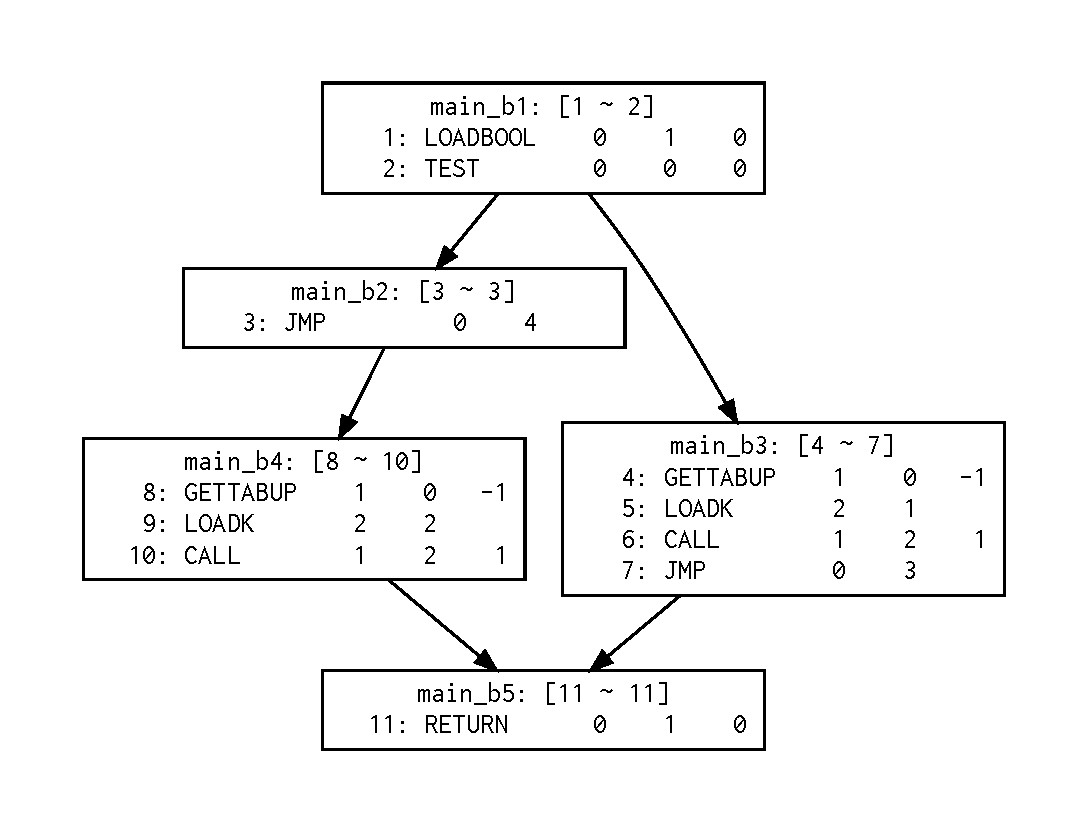
\includegraphics[width=1.3\textwidth]{img/cfg.pdf}
	\end{figure}
\end{minipage}
\end{frame}


\subsection{Optimizations}
\begin{frame}
	\frametitlesubs
	\begin{itemize}
		\item Constant Folding
		\item Constant Propagation
		\item Dead-Code Elimination
		\item Function Inlining
		\item Unreachable Block Removal
		\item Unused Resource Removal
	\end{itemize}
\end{frame}
\subsubsection{Constant Folding}
\begin{frame}[fragile]
	\frametitle{Constant Folding}

	\begin{enumerate}
		\item 演算命令のオペランドの型を調べて
		\item \lstinline{table}、\lstinline{userdata}\alert<2->{以外なら} \uncover<3->{$\Leftarrow$ \structure{メタメソッド}を考慮}
		\item 値を取ってきて
		\item 演算をおこない
		\item 即値命令にswap
	\end{enumerate}
\end{frame}
\subsubsection{Constant Propagation}
\begin{frame}[fragile]
	\frametitle{Constant Propagation}

	\begin{enumerate}
		\item \lstinline{MOVE}命令が参照してるregisterの定義位置を見て
		\item \lstinline{LOADK}なら\lstinline{MOVE}を\lstinline{LOADK}にする
	\end{enumerate}

	\pause
	\begin{itemize}
		\item 単体では速度改善なさそう
		\item \lstinline{LOADK}への依存が減るので、他の最適化を有利に進められる
		\item[] <3-> \textcolor{gray}{(今回の実装では)いまいちぱっとしない}
	\end{itemize}
\end{frame}
\subsubsection{Dead-Code Elimination}
\begin{frame}[fragile]
	\frametitle{Dead-Code Elimination}
	\begin{enumerate}
		\item \lstinline{LOADK}、\lstinline{MOVE}、\lstinline{CLOSURE}、\lstinline{LOADNIL}が生成するregistrの使用を調べ
		\item 0個の場合命令を消す
	\end{enumerate}

	\pause
	\begin{itemize}
		\item DU/UD Chainのわかりやすい使用例
	\end{itemize}
\end{frame}
\subsubsection{Function Inlining}
\begin{frame}[fragile]
	\frametitle{Function Inlining}
	\begin{enumerate}
		\item \lstinline{CALL}命令が引っ張ってくるclosureを見て
		\item 再帰関数でなければ展開
	\end{enumerate}
	\pause
	\begin{itemize}
		\item register windowの使用を抑えられる
		\item<3-> \alert{実は頼みの綱}
		\item<4-> バグがヤバい

			ア
	\end{itemize}
\end{frame}
\subsubsection{Unreachable Block Removal}
\begin{frame}
	\frametitle{Unreachable Block Removal}
	\begin{enumerate}
		\item 後続ブロックを持たない基本ブロックを丸々削除
		\item だけ
	\end{enumerate}
	\begin{itemize}
		\item 速くはならないがバイトコードのサイズ縮小に貢献
	\end{itemize}
\end{frame}
\subsubsection{Unused Resource Removal}
\begin{frame}
	\frametitle{Unused Resource Removal}
	\begin{enumerate}
		\item constant list、prototype listから不要なものを削除
		\item だけ
	\end{enumerate}
	\begin{itemize}
		\item 速くはならないがバイトコードのサイズ縮小に貢献
	\end{itemize}
\end{frame}


